\def\vector#1{\mbox{\boldmath $#1$}}

%!TEX root = ../thesis.tex
%*******************************************************************************
%****************************** Forth Chapter **********************************
%*******************************************************************************
\chapter[インターフェース]{インターフェース}
\graphicspath{{Chapters_implementation/Figs/}}



RealCodeは\ref{section:issue-classification}章で転用可能とされたイシューのデータを3種類のインターフェースを通じて演習問題として学習者に提供することができる.
図~\ref{fig:interface-selector},~\ref{fig:realcode-mobile}に示すように,システムはデスクトップとモバイルの両方に対応しており,ユーザの柔軟な学習を支援できる~\cite{gassler2004integrated}.
3種類のインターフェースはそれぞれ,単語帳(図~\ref{fig:flash}),選択式(図~\ref{fig:mcq}),穴埋め式(図~\ref{fig:fill})の形式で演習問題を提示する.
RealCodeではイシューの説明文を問題文として,対応するプルリクエストのコード変更を解答コードとして利用している.
現在のRealCodeには一般的なプログラミング言語(例,Python)に加えて,マークアップ言語(例,CSS)や拡張言語(例,Sass),設定言語(例,TOML)を含む51のプログラミング言語の演習問題が用意されている(但し,穴埋め式のインターフェースはPythonのみ).

\begin{figure}[H]
	\centering
  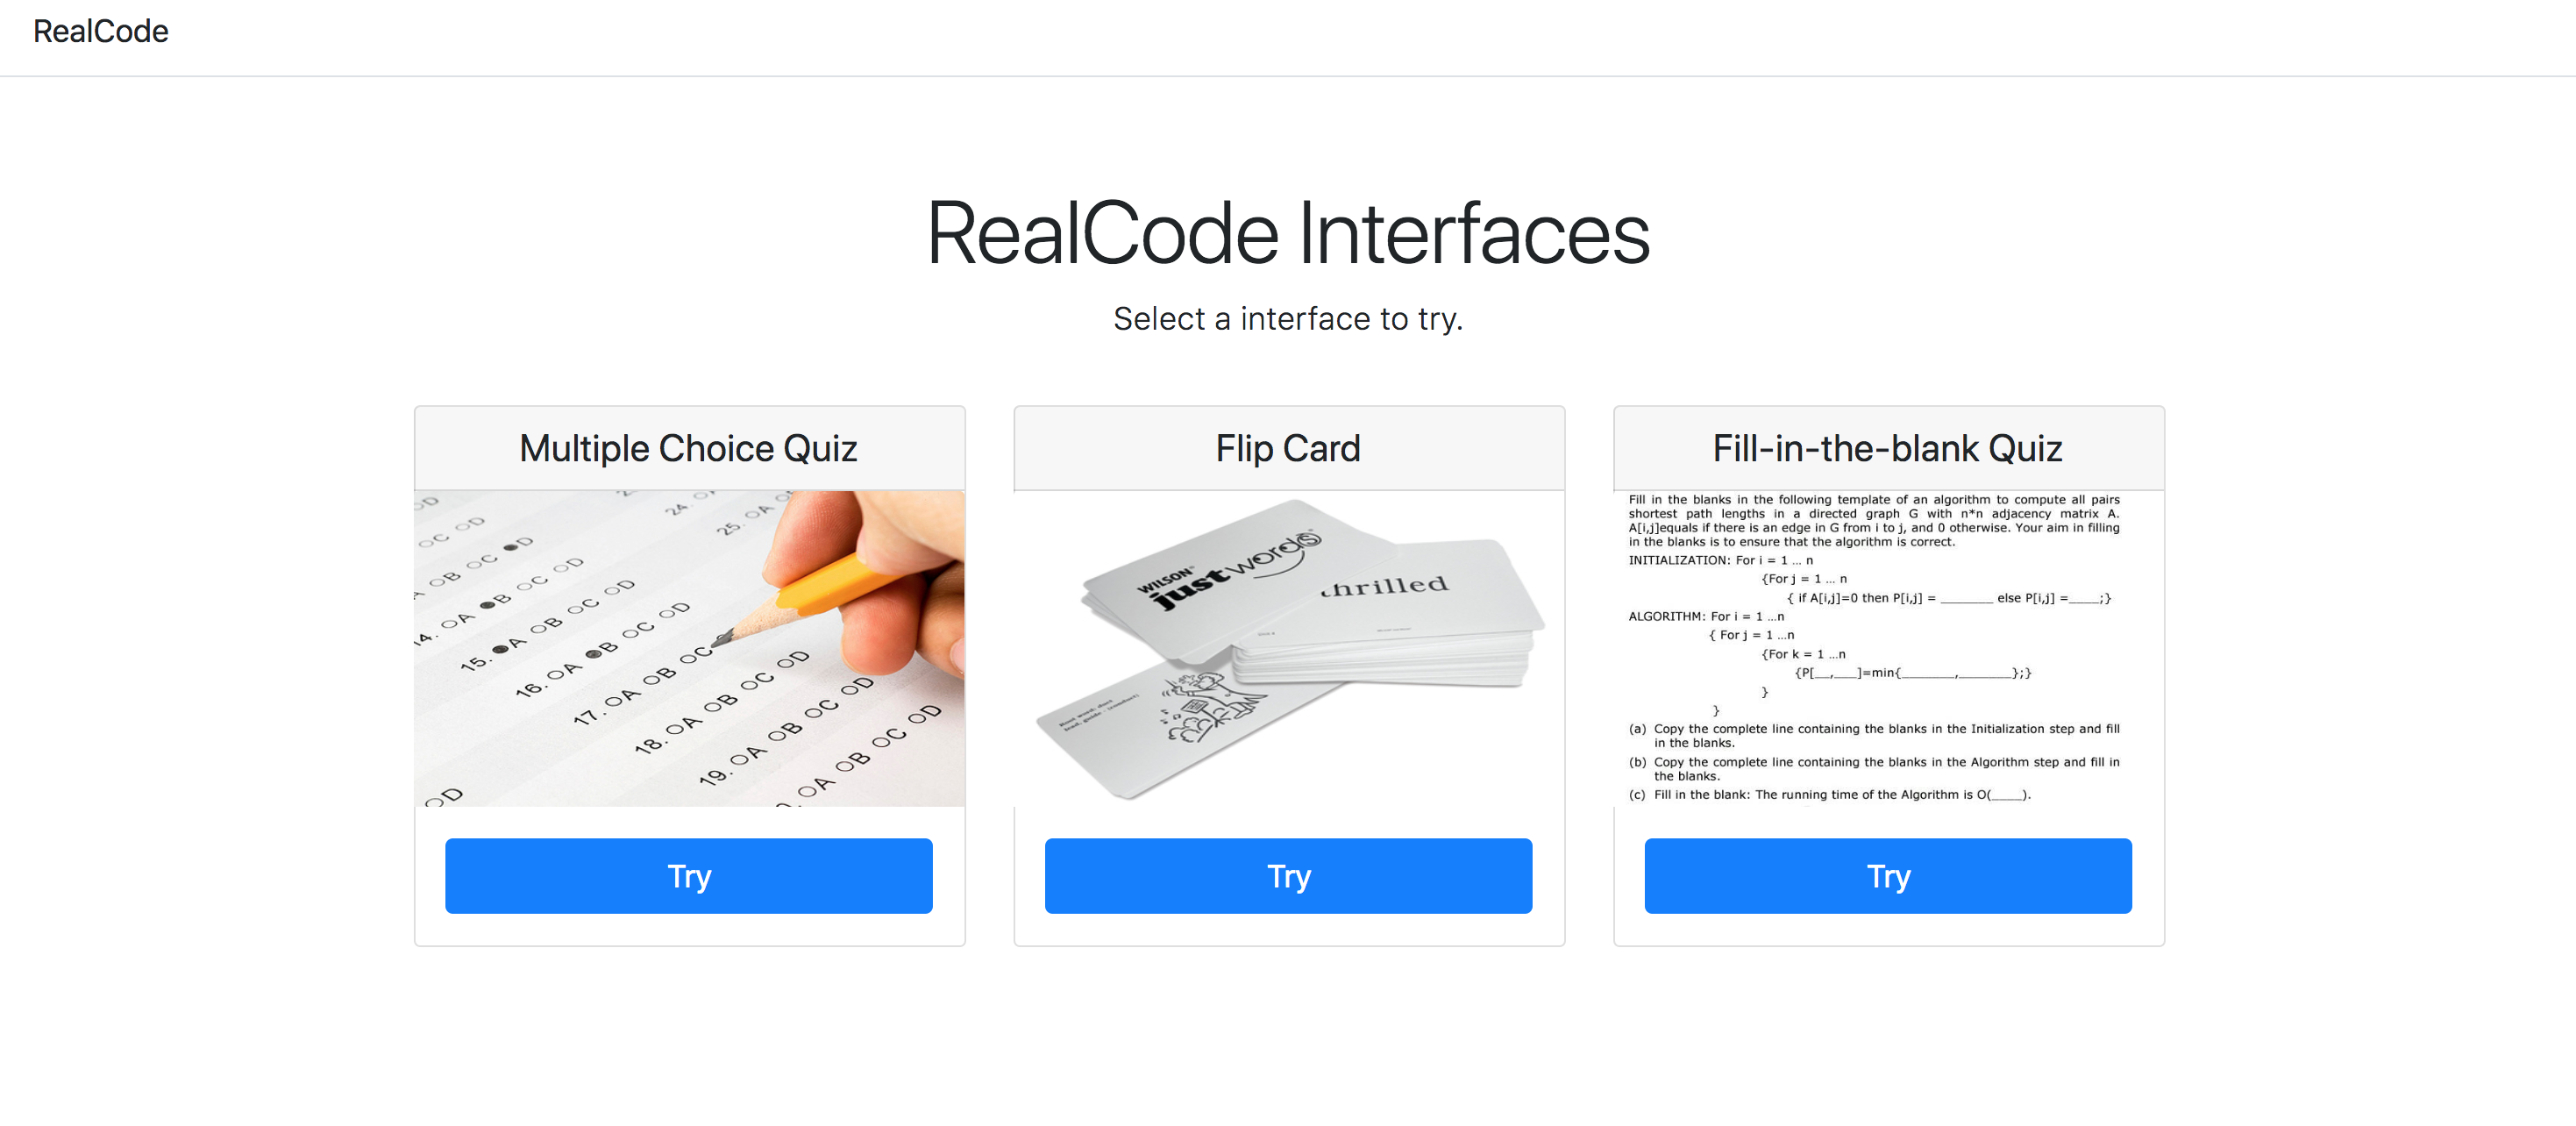
\includegraphics[width=1.0\columnwidth]{20181228-realcode-interfaces-select.png}
  \caption{デスクトップ版のRealCodeのインターフェース選択画面.}
  \label{fig:interface-selector}
\end{figure}

% \begin{figure}[H]
% 	\centering
%   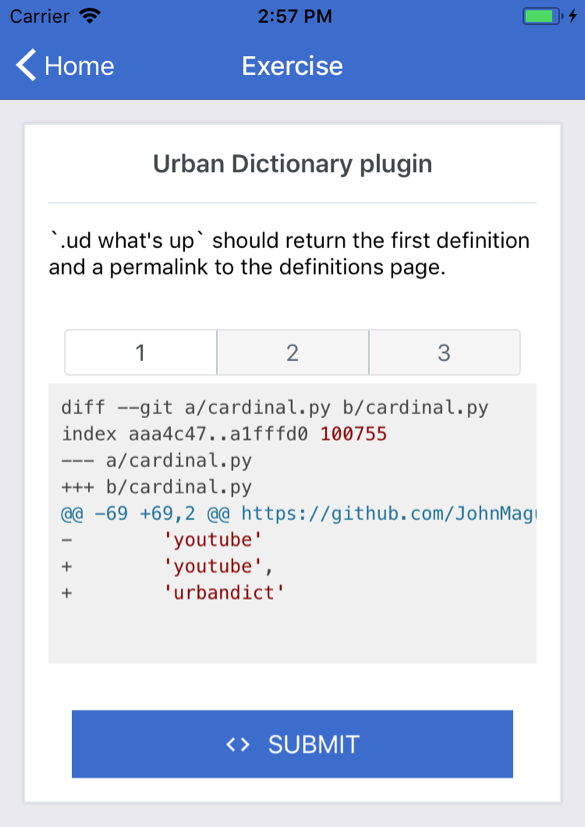
\includegraphics[width=1.0\columnwidth]{realcode_mobile.png}
%   \caption{モバイルのインターフェース.WIP.}
%   \label{fig:realcode-mobile}
% \end{figure}

\begin{figure}[H]
    \begin{tabular}{ccc}
      \begin{minipage}[t]{0.33\columnwidth}
        \centering
        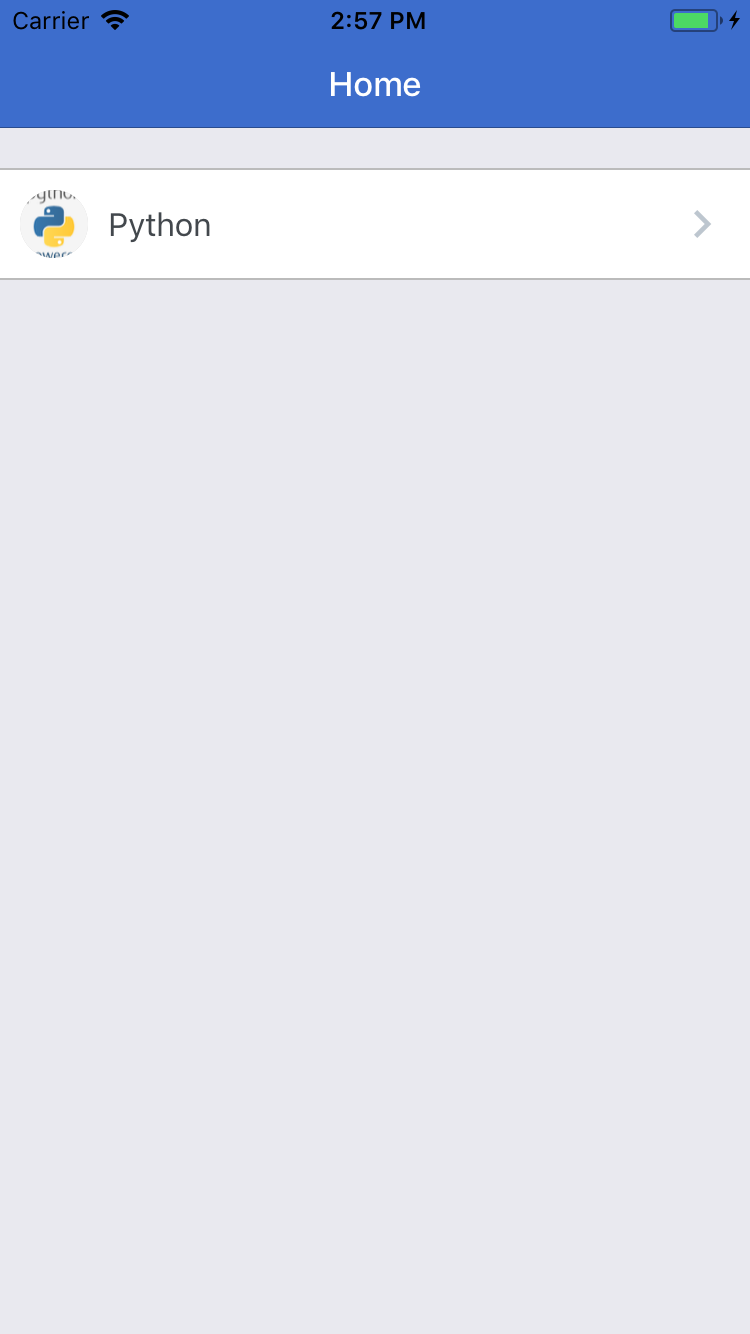
\includegraphics[width=1.0\columnwidth]{realcode-mobile-lang-selection.png}
        \subcaption{プログラミング言語の選択画面.}
      \end{minipage}
      \begin{minipage}[t]{0.33\columnwidth}
        \centering
        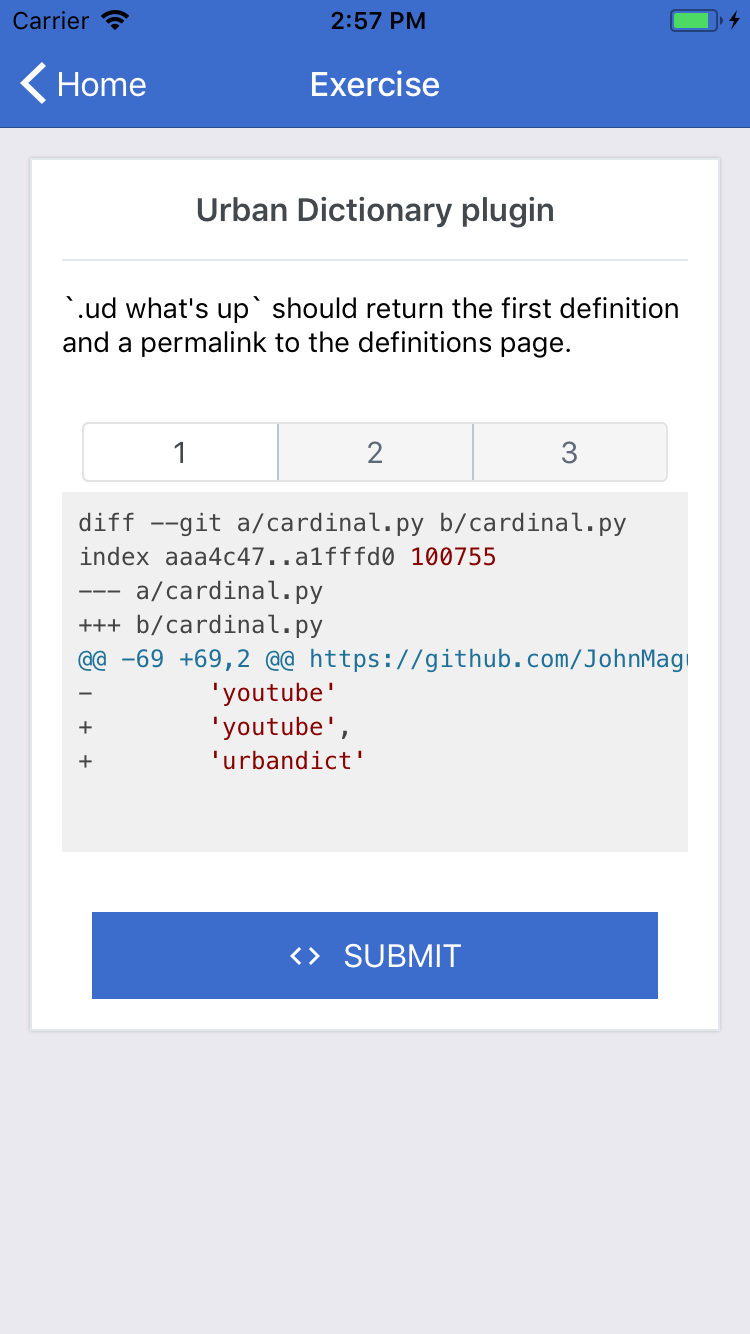
\includegraphics[width=1.0\columnwidth]{realcode-mobile-exercise.png}
        \subcaption{演習問題の画面.}
      \end{minipage}
      \begin{minipage}[t]{0.33\columnwidth}
        \centering
        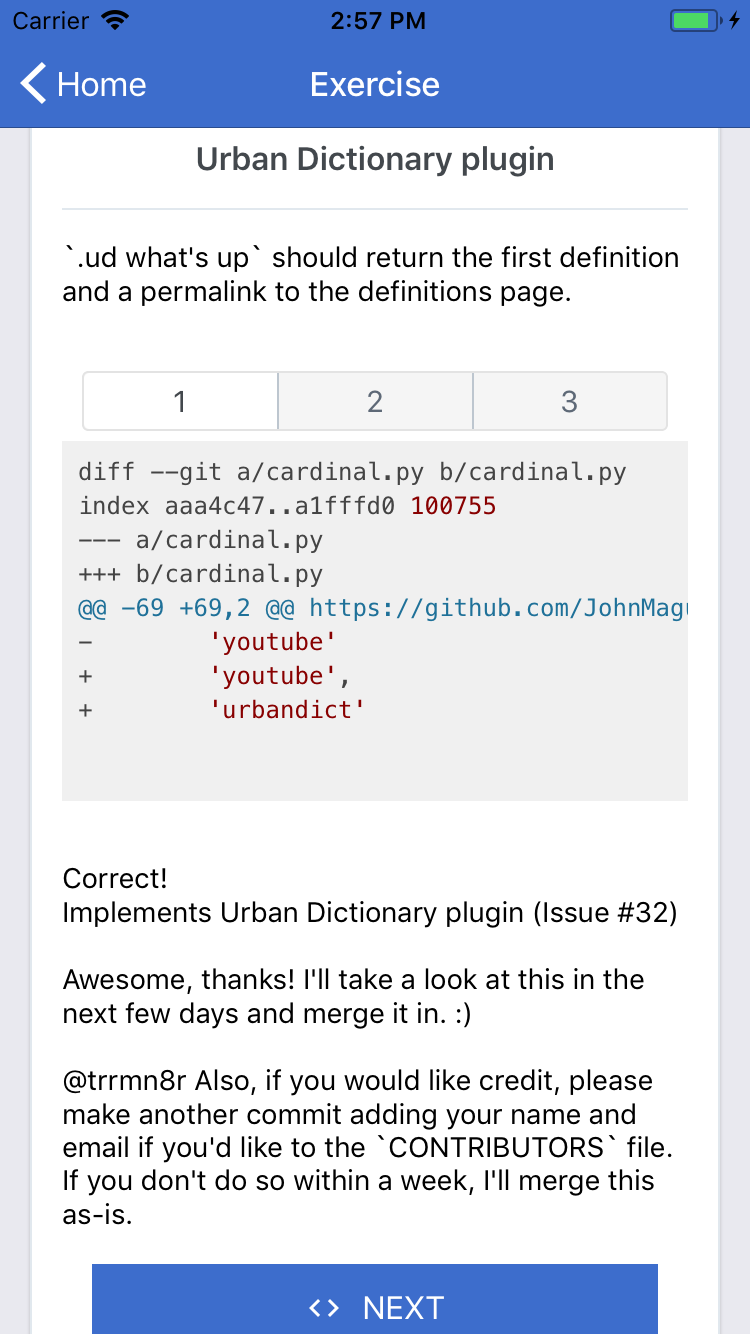
\includegraphics[width=1.0\columnwidth]{realcode-mobile-answer.png}
        \subcaption{演習問題の解答後の画面.}
      \end{minipage}
    \end{tabular}
    \caption{モバイル版のRealCodeのインターフェース.}
    \label{fig:realcode-mobile}
\end{figure}


\section{単語帳形式}

\begin{figure}[t]
    \begin{tabular}{cc}
      %---- Flip card, before ---------------------------
      \begin{minipage}[t]{1.0\columnwidth}
        \centering
        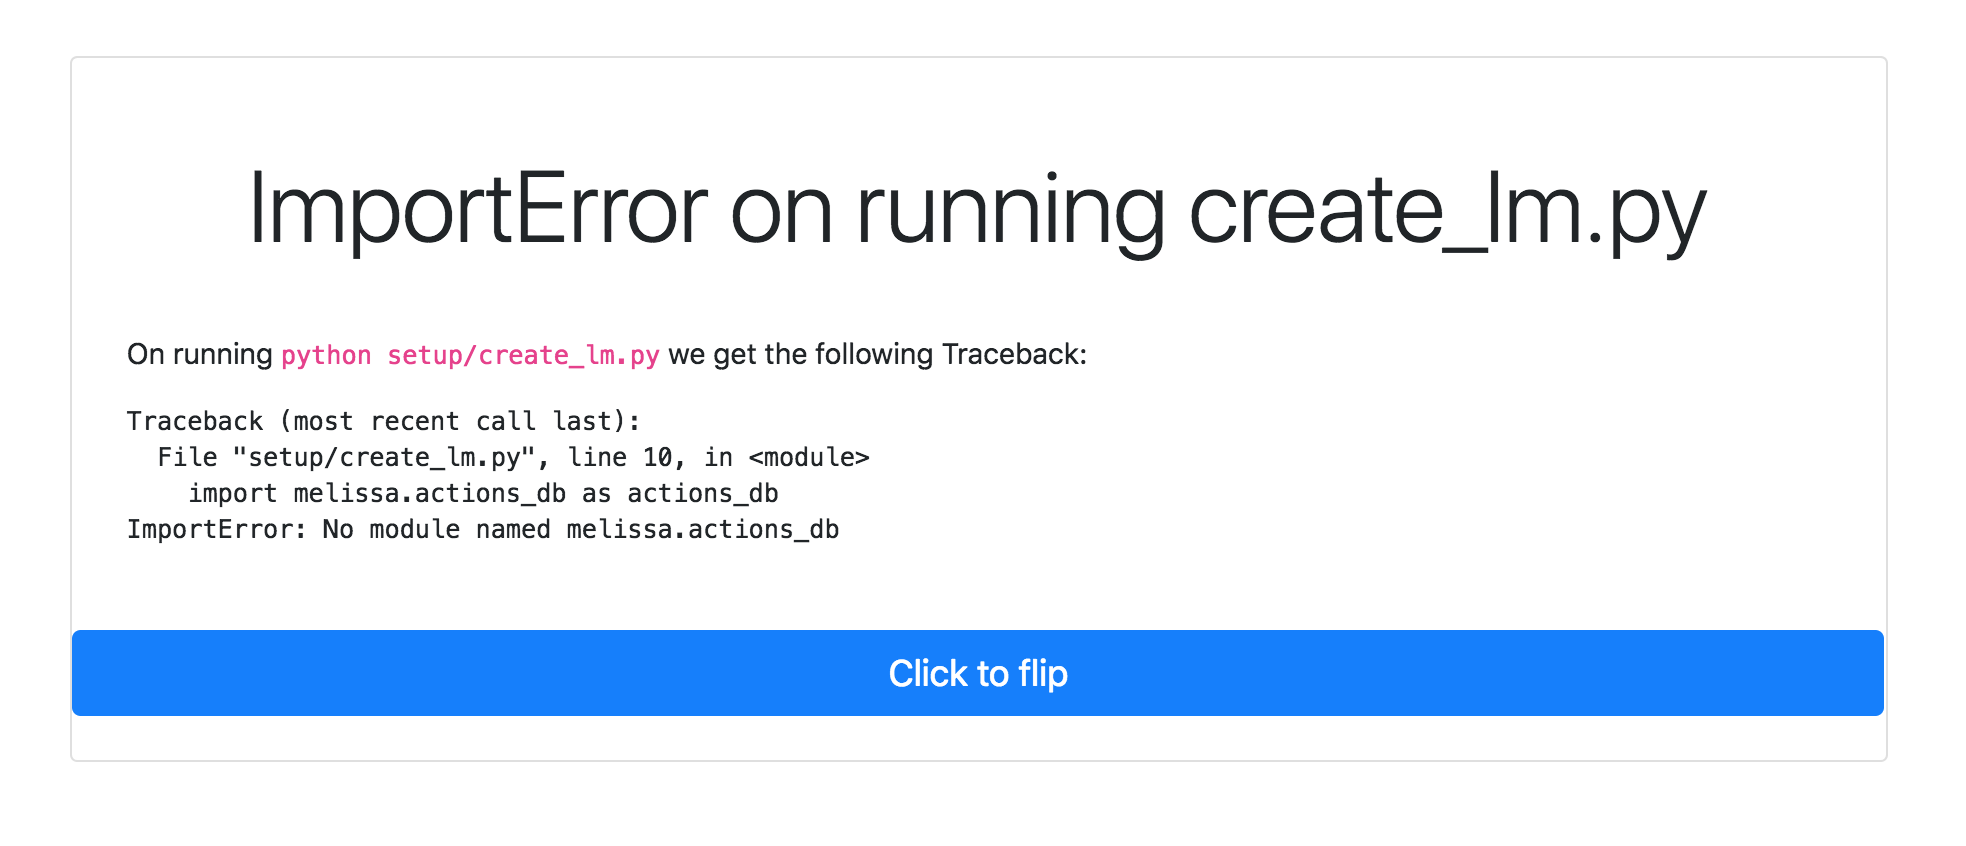
\includegraphics[width=1.0\columnwidth]{20181228-interface-flip-before.png}
        \subcaption{問題文側のインターフェース.}
        \label{fig:flash-before}
      \end{minipage} \\
      %---- Flip card, after --------------------------
      \begin{minipage}[t]{1.0\columnwidth}
        \centering
        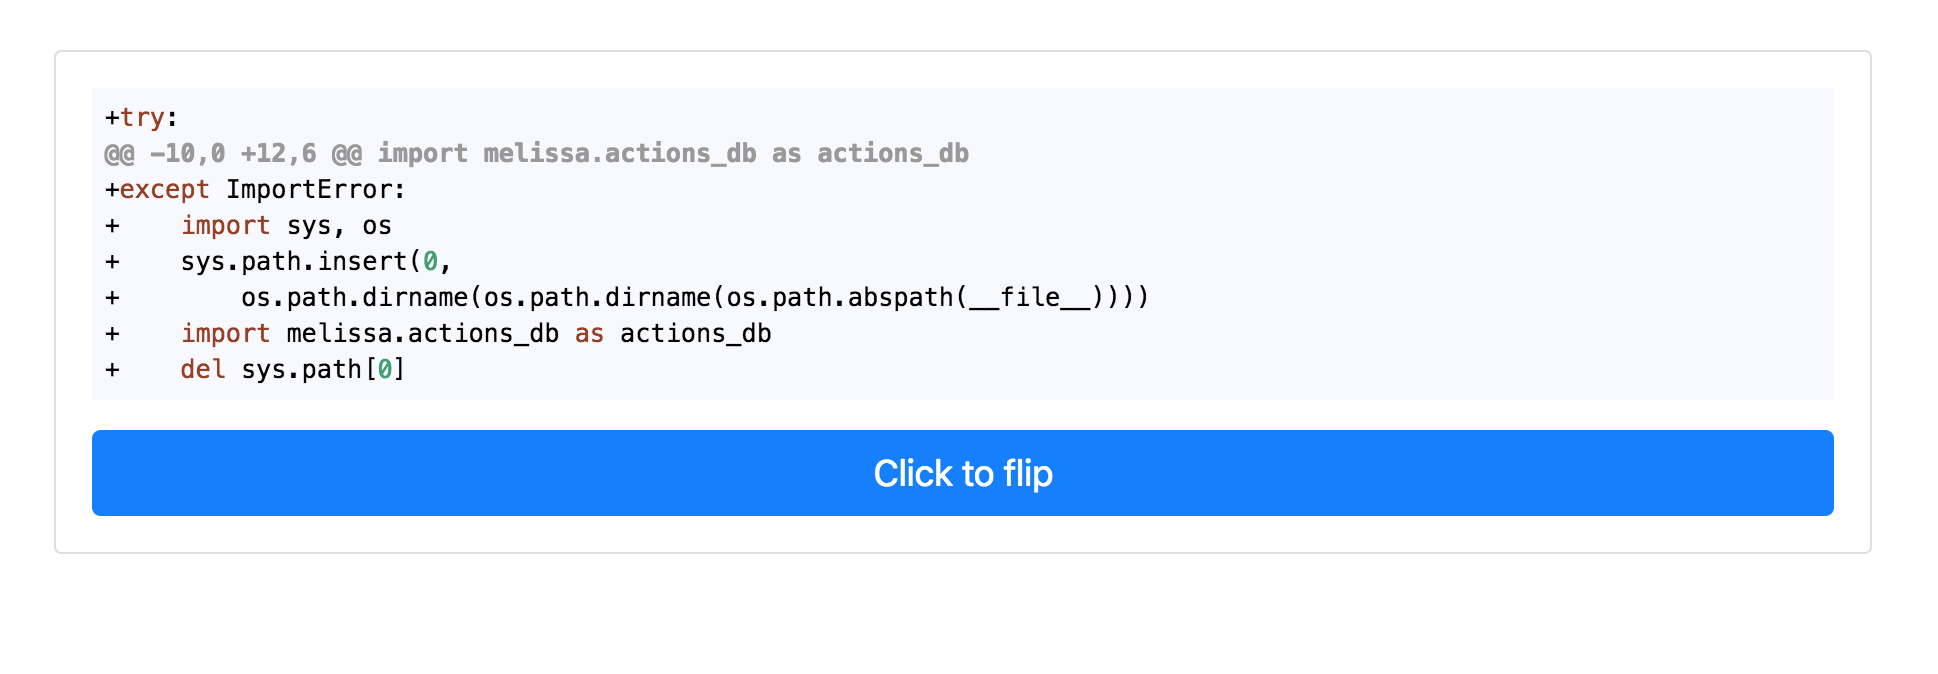
\includegraphics[width=1.0\columnwidth]{20181228-interface-flip-after.png}
        \subcaption{解答コード側のインターフェース.}
        \label{fig:flash-after}
      \end{minipage}
    \end{tabular}
    \caption{RealCodeの単語帳形式のインターフェース.``Click to flip''のボタンをクリックすることで,問題文と解答コードの画面を切り替えることができる.}
    \label{fig:flash}
\end{figure}

単語帳のようなフラッシュカードは繰り返し学習のための最も基本的な学習様式であり,特に反復による記憶に効果があることが確認されている~\cite{macquarrie2002comparison}.
図~\ref{fig:flash}に示すインターフェースにてユーザは問題文と解答コード見比べて読むことにより,演習問題の鍵となる構文(例,関数やAPIなど)を学習することを促す目的でこのインタフェースが提供されている.

% The \textit{FlashCard} interface is the most basic style for repeated learning~\cite{macquarrie2002comparison}.
% Users can simply review exercises and answer keys like flash cards.
% But unlike those for other purposes (e.g., vocabulary), it is not intended to make learners remember answer keys verbatim.
% Instead, learners are encouraged to examine what key components in the answer keys are (e.g., functions and APIs) and focus on remembering them.


\section{選択式}
\begin{figure}[t]
	\centering
  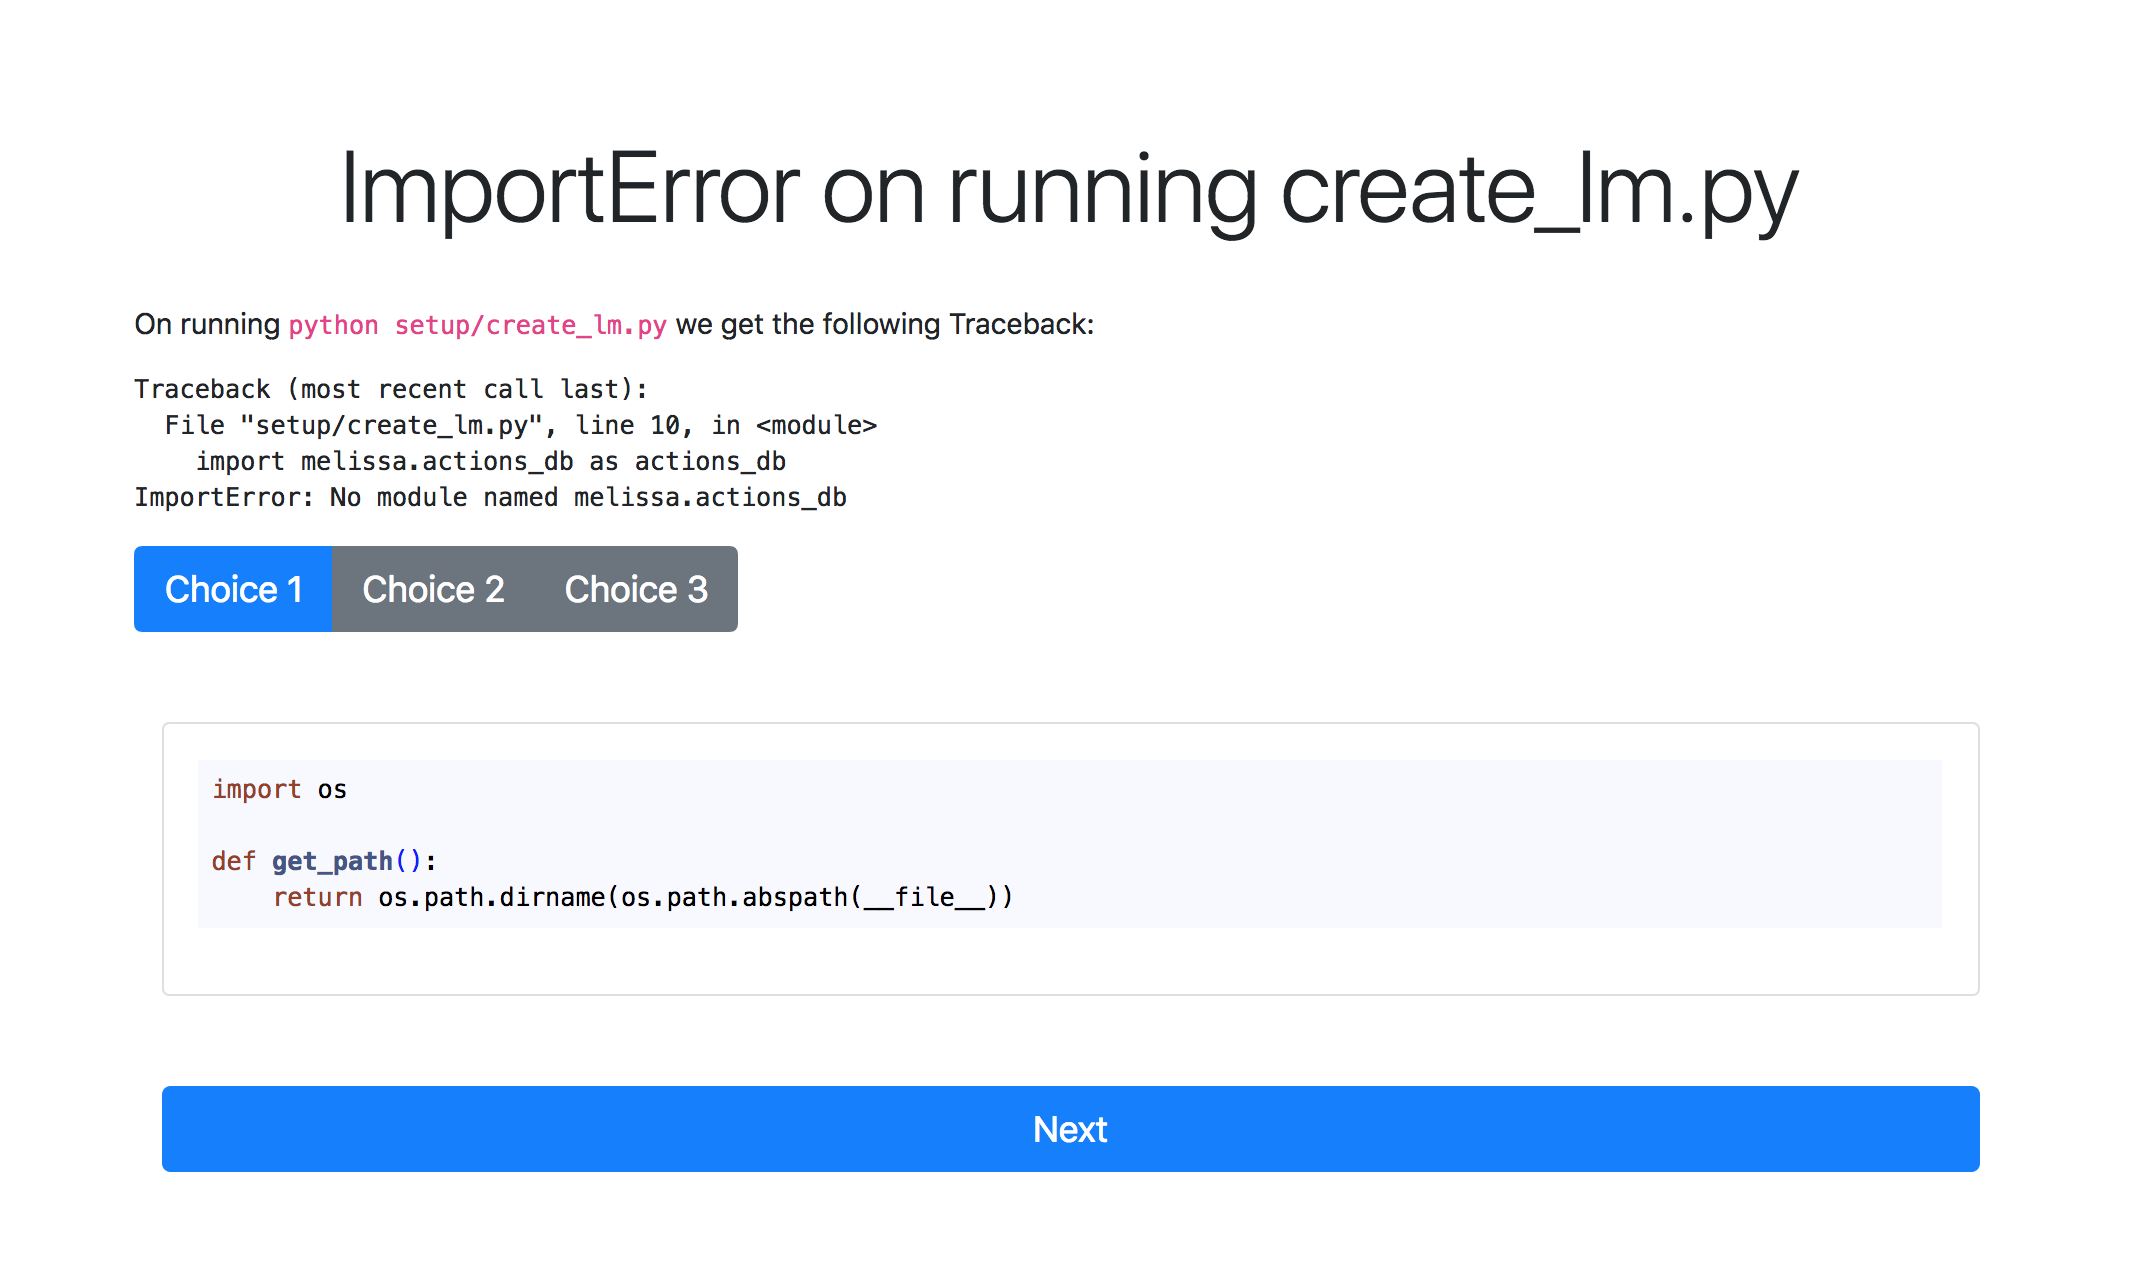
\includegraphics[width=1.0\columnwidth]{20181228-interface-mcq.png}
  \caption{RealCodeの選択式のインターフェース.``Choice~1'', ``Choice~2'', ``Choice~3''のボタンをクリックすると,解答の候補となる選択肢が表示される.}
  \label{fig:mcq}
\end{figure}

図~\ref{fig:mcq}に示す選択式のインターフェースでは,演習問題ごとに解答の候補となる複数の選択肢(3択)を提供する.
適度な難易度の演習問題にするためには,不正解の選択肢は正解の選択肢の解答コードと似ていながらも異なっている必要がある.
例えばコメントのみが異なる(正解とすべき正しく動作する)コードを不正解の選択肢として提示した場合,選択式の問題としては不適切となる.
そこで各演習問題につき2つの適切な不正解の選択肢を生成するために,我々はプログラミング言語ごとにコードの文字列的類似度の上限値を定め,上限値を超えない中で最も類似度の高いコードを不正解の選択肢として提供することとした.
その上限値の設定方法は以下の通りである.
はじめに上限値を仮に1と設定する.
次に,ランダムに選択された50問の演習問題の解答コードに対して,その他の全ての演習問題の解答コードとの文字列的類似度をword-level fuzzy matching~\cite{sankoff1983time}により計算する.
そして,上限値を超えない中で最も類似度の高かった2つのコードが,解答コード例とどの程度異なるかを著者らが判断した.
2つのコードが正解の選択肢と類似しすぎていた場合,上限値を0.05小さくしてから同様の処理を繰り返す.
以上の処理をプログラミング言語ごとに行うことで,上限値を決定している.
現在のプロトタイプでは上限値の決定を自動で行う事ができないため,自動的に上限値が決定できるようになればRealCodeの拡張性がさらに高まると考える.



\begin{figure}[tb]
    \begin{tabular}{cc}
      %---- Flip card, before ---------------------------
      \begin{minipage}[t]{0.95\columnwidth}
        \centering
        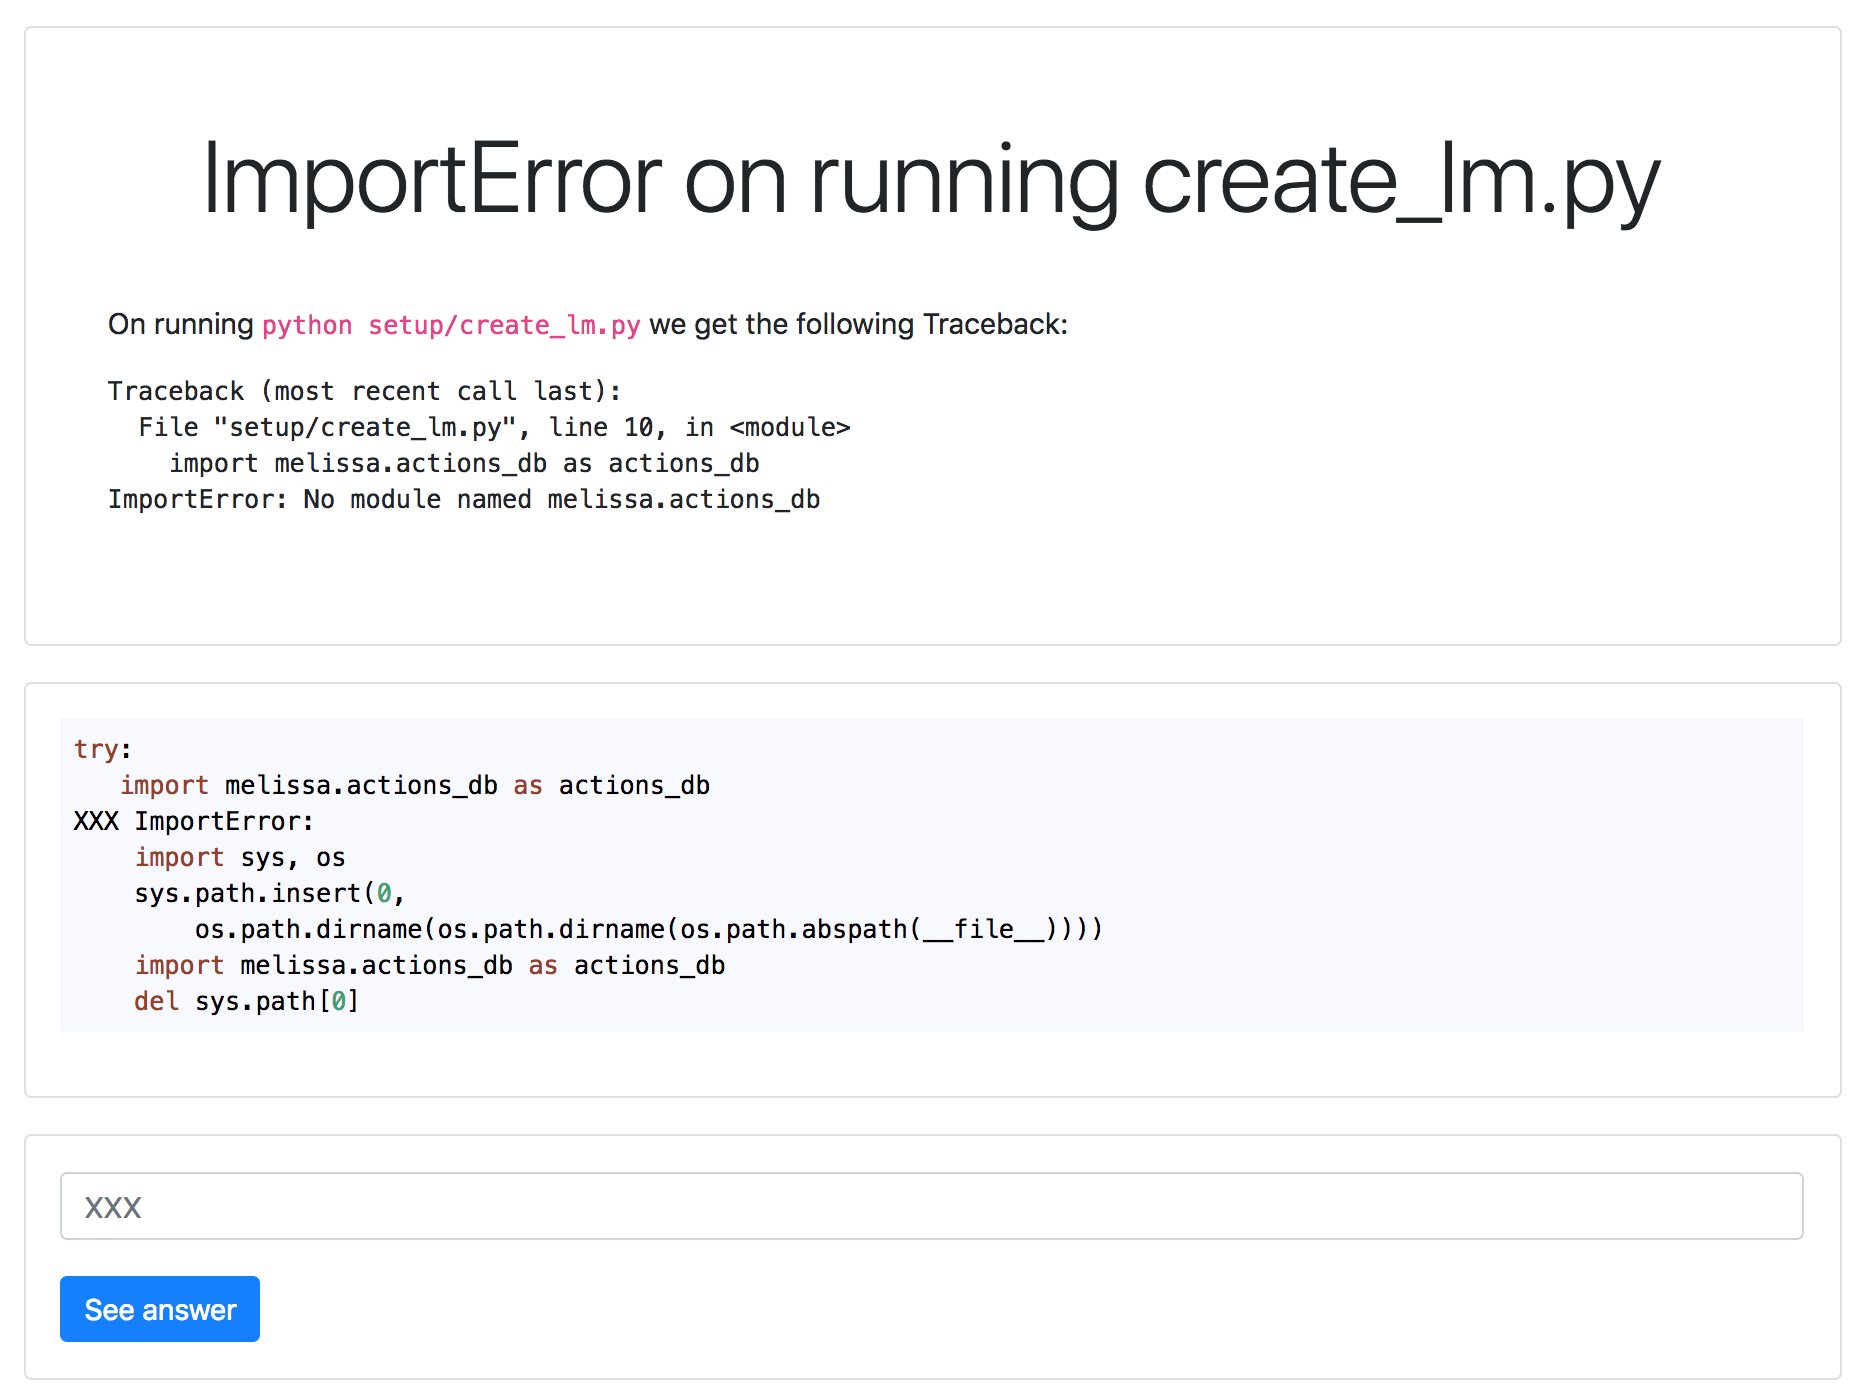
\includegraphics[width=0.9\columnwidth]{20181228-interface-fill-blank.png}
        \subcaption{回答前のインターフェース.ユーザは解答コード中の``XXX''に該当するPythonのコードを記述する.}
        \label{fig:fill-before}
      \end{minipage} \\ 
      %---- Flip card, after --------------------------
      \begin{minipage}[t]{0.95\columnwidth}
        \vspace{10 mm}
        \centering
        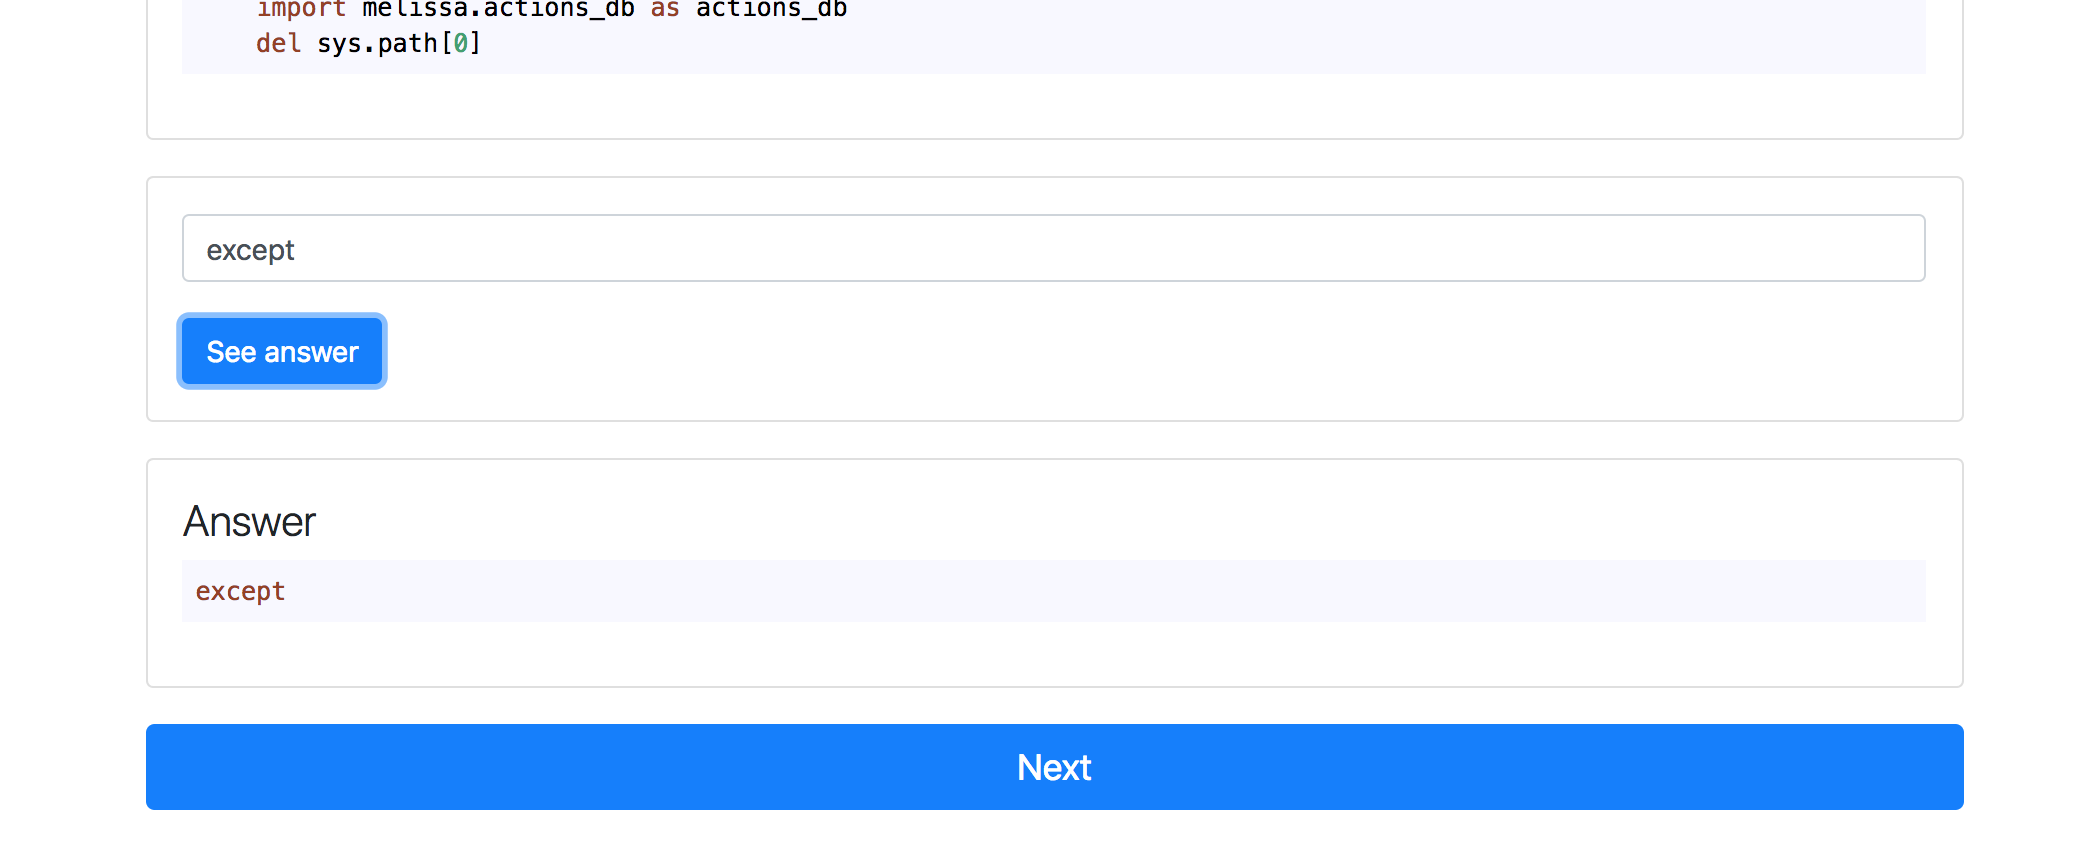
\includegraphics[width=1.0\columnwidth]{20181228-interface-fill-blank-after.png}
        \subcaption{回答後のインターフェース.}
        \label{fig:fill-after}
      \end{minipage}
    \end{tabular}
    \caption{RealCodeの穴埋め式のインターフェース.}
    \label{fig:fill}
\end{figure}

\section{穴埋め式}

図~\ref{fig:fill}に示す穴埋め式のインターフェースでは,ユーザは問題文を読んだ後に解答コード中の空欄に該当するPythonのコードを記述する(例,``for''や``except''など).
RealCodeはPythonで書かれた解答コードの構文木をあらかじめ作成し,その中からランダムに一か所を空欄とする.
現在のプロトタイプでは穴埋め式のインターフェースはPythonのみ対応しているが,構文解析を導入することで他のプログラミング言語にも対応することができる.
また,空欄とする構文をランダムでなくユーザが求める学習内容に応じて決定することができるようになれば,より体系的な学習体験を提供できるようになる可能性があると考える.

% The \textit{FillBlack} interface offers an advanced exercise by asking learners to fill a blank with a Python syntactic component (e.g., closures).
% Our system parses Python answer keys, and randomly selects one of components for a blank.
% Our current implementation supports this mode only in Python although extension to other languages is possible by integrating corresponding parsers.

